% !TEX root = memoire.tex

\tikzset{tuile/.style={draw, blue!60!black, fill=blue!10, minimum size=1cm, inner sep=0, outer sep=0}}
\newcommand{\tuile}[2][]{\node[tuile] at (#2) {#1}}

%\tikzset{point/.style={draw, circle, fill, inner sep=0.6mm}}
%\newcommand{\point}[1]{\node[point] at (#1) {}}
\newcommand{\point}[1]{\fill (#1) circle (3pt)}

\tikzset{pas/.style={auto, >=latex}}
\newcommand{\pas}[2]{\draw[pas] (#1) edge[->, bend left] (#2)}

% Typesetting gomino
\newcommand{\noir}{{\bf N}\xspace}
\newcommand{\blanc}{{\bf B}\xspace}

% Typesetting de Go

% Goban coté gauche
\newcommand{\goban}[2]{ 
	\clip (-0.7, -0.7) rectangle (#1.7-1,#2.7-1); 
	\fill[color=brown] (-0.7,-0.7) rectangle (#1,#2); 
	\draw (0,-1) grid (#1,#2+1); 
}

% Gobal central
\newcommand{\gobanc}[2]{ 
	\clip (-0.7, -0.7) rectangle (#1.7-1,#2.7-1); 
	\fill[color=brown] (-0.7,-0.7) rectangle (#1,#2); 
	\draw (-1,-1) grid (#1+1,#2+1); 
}

\newcommand{\kifu}[3][scale=.4]{
\begin{tikzpicture}[#1, every node/.style={#1, minimum size=1cm}, node distance=1cm]
\goban{#2}{#2}
#3
\end{tikzpicture}
}

\newcommand{\kifuc}[3][scale=1]{
\begin{tikzpicture}[#1, every node/.style={#1, minimum size=1cm}, node distance=1cm]
\gobanc{#2}{#2}
#3
\end{tikzpicture}
}


\newcommand{\woodgoban}[2]{
% parameters for the "wooden rectangle", chosen to be measures of a Go board
	\pgfmathsetmacro{\boardwidth}{#1}
	\pgfmathsetmacro{\boardheight}{#2}
	\pgfmathsetmacro{\relativefibrethickness}{0.10}
	\pgfmathsetmacro{\relativefibrevariation}{0.07}
	\pgfmathsetmacro{\numberoffibres}{(\boardwidth*5)} %20
	\pgfmathsetmacro{\fibresteps}{(\boardheight*5)} %10
	\newcommand{\backgroundcolor}{brown!95!yellow}
	\newcommand{\fibrecolor}{brown!95!black}

    %auto generated wood board  
	\clip (-0.7, -0.7) rectangle (\boardwidth + 0.7-1,\boardheight + 0.7-1); 

    \filldraw[\backgroundcolor] (-0.7, -0.7) rectangle (\boardwidth +0.7-1,\boardheight +0.7-1);

    \pgfmathsetmacro{\segmentwidth}{(\boardwidth + 0.7)/(\numberoffibres+1)}
    \pgfmathsetmacro{\segmentvariation}{\relativefibrethickness/2*\segmentwidth}

    \pgfmathsetmacro{\secondfibre}{2*\segmentwidth}
    \pgfmathsetmacro{\lastfibre}{\numberoffibres*\segmentwidth}

    \pgfmathsetmacro{\stepheight}{(\boardheight + 0.7)/\fibresteps}

	\begin{scope}[rotate=-2]
    \foreach \x in {0,...,\numberoffibres}
    {   \fill[\fibrecolor]
    			($(\x*\segmentwidth-\segmentvariation-0.7,0-0.7) + (rand*\relativefibrevariation*\relativefibrethickness,0)$) 
        
        		\foreach \y in {0,...,\fibresteps}
        		{
        			-- ($(\x*\segmentwidth-\segmentvariation-0.7,\y*\stepheight-0.7) + (rand*\relativefibrevariation*\relativefibrethickness,0)$)
        		}

	        -- ($(\x*\segmentwidth+\segmentvariation-0.7,\boardheight-0.7)+ (rand*\relativefibrevariation*\relativefibrethickness,0)$) 
    		    
    		    \foreach \y in {\fibresteps,...,0}
        		{   
        			-- ($(\x*\segmentwidth+\segmentvariation-0.7,\y*\stepheight-0.7) + (rand*\relativefibrevariation*\relativefibrethickness,0)$)
        		}
        -- cycle;
    }
    \end{scope}
	\draw (0,-1) grid (#1,#2+1); 
}


% Pierres
\newsavebox{\blackstonebox}
\savebox{\blackstonebox}{
	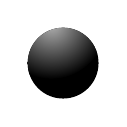
\begin{tikzpicture}
	\begin{scope}     	
		\fill[black] (0,0) circle (0.45);     	
		\clip (0,0) circle (0.45);     	
		\shade[outer color=black, inner color=black!30] (-0.15,0.5) circle (0.7); 	
	\end{scope}         
	\end{tikzpicture} 
}

\newsavebox{\whitestonebox}
\savebox{\whitestonebox}{
	
\begin{tikzpicture}
	\begin{scope}     	
		\fill[white!80!black] (0,0) circle (0.45);   
		\clip (0,0) circle (0.45);     	
		\shade[outer color=white!80!black, inner color=white] (-0.15,0.5) circle (0.7); 	
	\end{scope}         
	\end{tikzpicture} 
}

\newsavebox{\redstonebox}
\savebox{\redstonebox}{
	
\begin{tikzpicture}
	\begin{scope}        
		\fill[red] (0,0) circle (0.45);        
		\clip (0,0) circle (0.45);        
		\shade[outer color=red, inner color=red!30] (-0.15,0.5) circle (0.7);        
	\end{scope}
	\end{tikzpicture}
}

\newsavebox{\customwalkbox}
\savebox{\customwalkbox}{
	
\begin{tikzpicture}
	\fill (0,0) rectangle (1,1);
	\end{tikzpicture}
}

\newcommand{\blackstone}{ \usebox{\blackstonebox} }
\newcommand{\whitestone}{ \usebox{\whitestonebox} }
\newcommand{\redstone}{ \usebox{\redstonebox} }
\newcommand{\customwalknode}{\usebox{\customwalkbox}}

\newcommand{\bm}[2][]{ \node at #2 {\blackstone}; \node at #2 {\color{white} #1}; }
\newcommand{\wm}[2][]{ \node at #2 {\whitestone}; \node at #2 {\color{black} #1};}


\usepackage{etextools}

% Using etextools, create a parser without delimiters that will 
% tokenize and process each letter one by one
\DeclareListParser*{\wordpath}{}

% Our substitution to convert the word to a TikZ path
\newcommand\BlackWalkParser[1]{
\ifcase \gettokslistindex{#1}{01234567} 
{--++(1,0) node{\blackstone} }
\or {--++(1,1) node{\blackstone} }
\or {--++(0,1) node{\blackstone} }
\or {--++(-1,1) node{\blackstone} }
\or {--++(-1,0) node{\blackstone} }
\or {--++(-1,-1) node{\blackstone} }
\or {--++(0,-1) node{\blackstone} }
\or {--++(1,-1) node{\blackstone} }
\fi}

\newcommand\WhiteWalkParser[1]{
\ifcase \gettokslistindex{#1}{01234567} 
{--++(1,0) node{\whitestone} }
\or {--++(1,1) node{\whitestone} }
\or {--++(0,1) node{\whitestone} }
\or {--++(-1,1) node{\whitestone} }
\or {--++(-1,0) node{\whitestone} }
\or {--++(-1,-1) node{\whitestone} }
\or {--++(0,-1) node{\whitestone} }
\or {--++(1,-1) node{\whitestone} }
\fi}

\newcommand\CustomWalkParser[1]{
\ifcase \gettokslistindex{#1}{01234567} 
{--++(1,0) node{\customwalknode} }
\or {--++(1,1) node{\customwalknode} }
\or {--++(0,1) node{\customwalknode} }
\or {--++(-1,1) node{\customwalknode} }
\or {--++(-1,0) node{\customwalknode} }
\or {--++(-1,-1) node{\customwalknode} }
\or {--++(0,-1) node{\customwalknode} }
\or {--++(1,-1) node{\customwalknode} }
\fi}

\newcommand\SimplePathParser[1]{
\ifcase \gettokslistindex{#1}{01234567} 
{--++(1,0)}
\or {--++(1,1)}
\or {--++(0,1)}
\or {--++(-1,1)}
\or {--++(-1,0)}
\or {--++(-1,-1)}
\or {--++(0,-1)}
\or {--++(1,-1)}
\fi}


% a command to invoke the parser and do the substitution
\newcommand\blackwalk[1]{\wordpath{\BlackWalkParser}{#1}}
\newcommand\whitewalk[1]{\wordpath{\WhiteWalkParser}{#1}}
\newcommand\customwalk[1]{\wordpath{\CustomWalkParser}{#1}}
\newcommand\simplewalk[1]{\wordpath{\SimplePathParser}{#1}}

% one-step parsing/drawing.
\newcommand\whitestonepath[2]{
	\edef\tmp{\whitewalk{#2}};
	\path #1 node{\whitestone} \tmp;
}

\newcommand\blackstonepath[2]{
	\edef\tmp{\blackwalk{#2}};
	\path #1 node{\blackstone} \tmp;
}

\newcommand\custompath[2]{
	\edef\tmp{\customwalk{#2}};
	\path #1 node{\customwalknode} \tmp;
}


\newcommand{\squarepath}[3][blue]{
	\savebox{\customwalkbox}{\draw[#1!60!black, fill=#1!10] (0,0) rectangle (1,1);}
	\custompath{#2}{#3};
}

\newcommand\simplepath[3][]{
	\edef\tmp{\simplewalk{#3}};
	\draw[#1] #2 \tmp;
}

\newcommand{\expandboundingbox}{\node[inner sep=0] at ($(current bounding box.north east) + (1,1)$) {};}
\newcommand{\polyomino}[2][blue]{
\begin{tikzpicture}[fill=red]
\squarepath[#1]{(0,0)}{#2}
\expandboundingbox
\end{tikzpicture}
}

%
% Example
%
%\begin{tikzpicture}
%\squarewalk{(0,1)}{000222};
%\squarewalk[red]{(0,0)}{00066};
%\end{tikzpicture}

% Paul Gaborit
% http://tex.findincity.net/view/635399273629833626147690/tikz-radial-shading-of-a-ring
\tikzset{
  ring shading/.code args={from #1 at #2 to #3 at #4}{
    \pgfmathsetmacro{\inner}{25*#2/#4}
    \pgfmathsetmacro{\innerlow}{\inner-1}
    \pgfdeclareradialshading{ring}{\pgfpoint{0cm}{0cm}}%
    {
      color(0bp)=(white);
      color(\innerlow bp)=(white);
      color(\inner bp)=(#1);
      color(25bp)=(#3);
      color(50bp)=(black)
    }
    \pgfkeysalso{/tikz/shading=ring}
  },
}

\pgfdeclareradialshading{stoneshading}{\pgfpointorigin}
{
  color(0mm)=(pgftransparent!100);
  color(0.45cm)=(pgftransparent!0);
  color(0.4501cm)=(pgftransparent!30);
  color(.6cm)=(pgftransparent!100)
}
\pgfdeclarefading{stonemarking}{\pgfuseshading{stoneshading}}
\pgfdeclarefading{fading3}{\pgfuseshading{stoneshading}}

\newcommand{\markstone}[3][green]{
\begin{scope}
\pgfsetfading{stonemarking}{\pgftransformshift{\pgfpoint{#2cm}{#3cm}}};
\fill [#1, even odd rule] (#2, #3) circle (.6) circle (.45);
\end{scope}
}